\chapter{Arhitektura i dizajn sustava}
		
		Arhitektura se može podijeliti na dva podsustava:
	\begin{itemize}
		\item Mobilna aplikacija
		\item Baza podataka
	\end{itemize}
	
	\begin{figure}[h]
		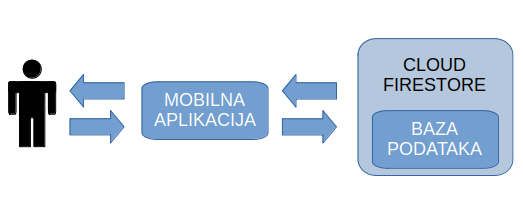
\includegraphics[scale=0.55]{slike/Arhitektura_sustava.PNG}
		\centering
		\caption{Arhitektura sustava}
		\label{fig:Arhitektura_sustava}
	\end{figure}
	
		\textit{\underbar{Mobilna aplikacija}} je program koji se izvodi na mobilnom uređaju. Mobilne aplikacije se uglavnom preuzimaju s distribucijskih platformi, nakon čega se provodi njihova instalacija. Korisnik koristi mobilnu aplikaciju za obrađivanje željenih zahtjeva, pri čemu aplikacija po potrebi pristupa bazi podataka.
		
		\textit{\underbar{Baza podatka}} je organizirani skup strukturiranih podataka. Za pohranu i pristup podacima koristi se računalni sustav.
		
		Za izradu naše mobilne aplikacije odabrali smo \href{https://flutter.dev/}{\textbf{Flutter}}, softver za razvoj korisničkog sučelja otvorenog koda koji je stvorio Google. Razlog zbog kojeg smo odabrali Flutter je jednostavnost izrade aplikacija i mogućnost višeplatformskog razvoja korištenjem jednog koda. Još jedna velika prednost je ta što se njime može realizirati i frontend i backend. Flutter koristi programski jezik Dart. Odabrano razvojno okruženje je Visual Studio Code.
		
		Baza podataka koju ćemo koristiti je \href{https://firebase.google.com/docs/firestore}{\textbf{Cloud Firestore}}. Cloud Firestore je NoSQL, dokumentno orijentirana baza podataka. Dokumenti su organizirani u kolekcije, a svaki dokument ima svoje ime (koje služi kao identifikator) i skup atributa kojima su pridružene vrijednosti. Glavne prednosti ovakve organizacije su efikasni upiti i velika brzina rada. Cloud Firestore omogućuje iOS, Android i web aplikacijama izravan pristup putem njihovih vlastitih programskih alata.
		
		Arhitektura sustava temeljiti će se na MVVM (Model-View-ViewModel) konceptu. Karakteristika MVVM koncepta je podjela na komponente čiji nezavisni razvoj osigurava fleksibilnost, smanjuje međuovisnost, povećava ponovnu uporabivost i pojednostavljuje ispitivanje. \newline
		MVVM koncept se sastoji od:
	\begin{itemize}
		\item \textbf{\underline{Model}} - Pohranjuje podatke i informacije potrebne za rad aplikacije. Odvojen je od logičkog dijela koji određuje prikaz podataka i usluga koje njima manipuliraju.
		\item \textbf{\underline{View}} - Predstavlja sučelje koje korisnik vidi u interakciji s aplikacijom. Identificira i reagira na korisničke akcije.
		\item \textbf{\underline{ViewModel}} - Središnja komponenta sustava. Služi kao sučelje između Modela i Viewa. Šalje i prima podatke od Modela te osigurava podatke potrebne Viewu. Također, promatra promjene koje se događaju u Viewu. Raspolaže metodama koje održavaju stanja Viewa i upravlja podacima u Modelu.
	\end{itemize}
		
	\eject

				
		\section{Baza podataka}
			
			\text Za potrebe našeg sustava koristit ćemo NoSQL bazu podataka orijentiranu na dokumente, odnosno kolekcije dokumenata. Gradivna jedinka baze je dokument koji je definiran svojim imenom i skupom atributa. Zadaća baze podataka jest jednostavna i brza pohrana, izmjena i dohvat podataka za daljnju obranu. Baza podataka ove aplikacije sastoji se od tri entiteta, a to su:
			
			\begin{itemize}
				\item User
				\item Categories
				\item Meetings
			\end{itemize}
		
			\subsection{Opis tablica}
			

				\textbf{User} \text    Ovaj entitet sadržava sve važne informacije o korisniku aplikacije. Sadrži atribute: about, cardExp, creditCard, firstName, iban, image, lastName, lecturer, mail, secCode, username. Za svakog novog registriranog korisnika kreira se dokument pod šifrom u bazi podataka.
				
				\begin{longtabu} to \textwidth {|X[6, l]|X[6, l]|X[20, l]|}
					
					\hline \multicolumn{3}{|c|}{\textbf{User}}	 \\[3pt] \hline
					\endfirsthead
					
					\hline \multicolumn{3}{|c|}{\textbf{User}}	 \\[3pt] \hline
					\endhead
					
					\hline 
					\endlastfoot
					
					Mail & string & mail korisnika \\ \hline
					Username & string & korisničko ime \\ \hline
					Lecturer & boolean & oznaka je li korisnik registriran kao predavač \\ \hline
					FirstName & string & ime korisnika \\ \hline
					LastName & string & prezime korisnika \\ \hline
					CardExp & string & datum isteka kartice za naplatu \\ \hline
					CreditCard & string & broj kartice za naplatu \\ \hline
					SecCode & string & kod za verifikaciju kartice \\ \hline
					iban & string & IBAN računa za isplatu honorara \\ \hline
					About & string & kratka biografija o korisniku ukoliko je predavač \\ \hline
					Image & string & poveznica na fotografiju korisnika ukoliko je predavač \\ \hline
					Courses & array & sadrži sve tečajeve koje je korisnik upisao (za polaznika) ili koje je kreirao (za predavača) \\ \hline					
				\end{longtabu}
			
			\textbf{Categories} \text    Ovaj entitet sadržava sve važne informacije o tečajevima koji su dostupni na aplikaciji. Sadrži atribut name te kolekciju za svaku razinu tečaja (beginner, intermediate, advanced) koja će sadržavati dodatne informacije o pojedinom tečaju. Za svaku kategoriju tečaja kreiran je dokument u bazi podataka, a za svaki tečaj kreira se dokument unutar kolekcije za odrabranu razinu i kategoriju tečaja. 
			
			\begin{longtabu} to \textwidth {|X[6, l]|X[6, l]|X[20, l]|}
				
				\hline \multicolumn{3}{|c|}{\textbf{Categories}}	 \\[3pt] \hline
				\endfirsthead
				
				\hline \multicolumn{3}{|c|}{\textbf{Categories}}	 \\[3pt] \hline
				\endhead
				
				\hline 
				\endlastfoot
				
				Name & string & naziv kategorije tečaja \\ \hline
				Difficulty & kolekcija & sadrži tri moguće razine tečajeva: početnička, srednja i napredna \\ \hline					
				
			\end{longtabu}
		
			\textbf{Difficulty} \text    Ova kolekcija unutar entiteta Courses sadrži kolekcije tečajeva (pod određenom kategorijom) raspoređene po razinama. 
			
			\begin{longtabu} to \textwidth {|X[6, l]|X[6, l]|X[20, l]|}
				
				\hline \multicolumn{3}{|c|}{\textbf{Difficulty}}	 \\[3pt] \hline
				\endfirsthead
				
				\hline \multicolumn{3}{|c|}{\textbf{Difficulty}}	 \\[3pt] \hline
				\endhead
				
				\hline 
				\endlastfoot
				
				Beginner & kolekcija & početnička razina tečaja \\ \hline
				Advanced & kolekcija & napredna razina tečaja \\ \hline
				Intermediate & kolekcija & srednja razina tečaja \\ \hline					
				
			\end{longtabu}
		
		
				\textbf{Beginner/Advanced/Intermediate} \text    Ove kolekcije sadrže informacije o tečaju koje su nužne za njegovo kreiranje. 
			
			\begin{longtabu} to \textwidth {|X[8, l]|X[6, l]|X[20, l]|}
				
				\hline \multicolumn{3}{|c|}{\textbf{Beginner/Advanced/Intermediate}}	 \\[3pt] \hline
				\endfirsthead
				
				\hline \multicolumn{3}{|c|}{\textbf{Beginner/Advanced/Intermediate}}	 \\[3pt] \hline
				\endhead
				
				\hline 
				\endlastfoot
				
				CourseInfo & string & kratki opis tečaja (do 1000 riječi) \\ \hline
				CourseMail & string & e-mail adresa vlasnika tečaja \\ \hline
				CourseMaterials & array & materijali za učenje (PDF format do 50 MB ukupno) \\ \hline
				CourseName & string & naziv tečaja \\ \hline
				CoursePrice & number & cijena tečaja \\ \hline
				Keywords & array & ključne riječi po kojima je moguće pronaći tečaj \\ \hline
								
				
			\end{longtabu}
		\eject
		
			\textbf{Meetings} \text    Ovaj entitet sadržava sve važne informacije o zatraženim konzultacijama. 
			
			\begin{longtabu} to \textwidth {|X[9, l]|X[6, l]|X[20, l]|}
				
				\hline \multicolumn{3}{|c|}{\textbf{Meetings}}	 \\[3pt] \hline
				\endfirsthead
				
				\hline \multicolumn{3}{|c|}{\textbf{Meetings}}	 \\[3pt] \hline
				\endhead
				
				\hline 
				\endlastfoot
				
				CourseID & string & ID dokumenta u bazi podataka za odabrani tečaj  \\ \hline
				LecturerConfirm & boolean & oznaka da je predavač potvrdio termin konzultacija \\ \hline
				LecturerMail & string & e-mail predavača \\ \hline
				ReqDate & string & traženi datum konzultacija \\ \hline
				StudentConfirm & boolean & oznaka da je polaznik potvrdio termin konzultacija \\ \hline
				StudentMail & string & e-mail polaznika koji je zatražio konzultacije \\ \hline				
				
			\end{longtabu}
			\pagebreak
			
			\subsection{Dijagram baze podataka}
				\begin{figure}[H]
					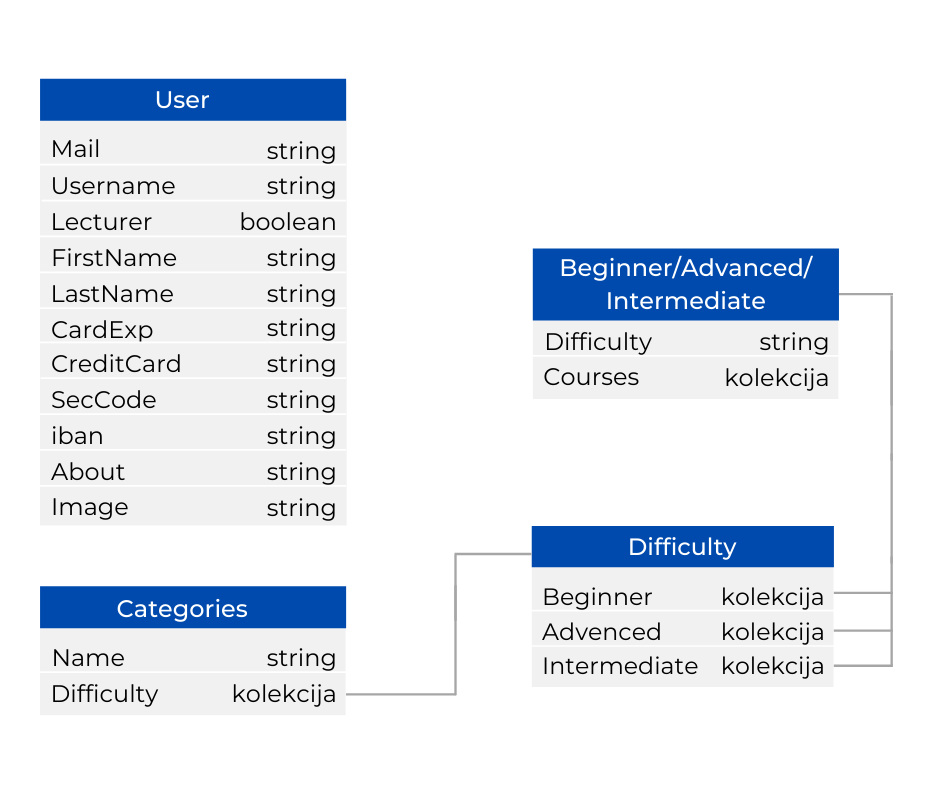
\includegraphics[scale=0.6]{dijagrami/ER_baza_podataka.PNG} 
					\centering
					\caption{E-R dijagram baze podataka}
					\label{fig:ER}
				\end{figure} 
			
			\eject
			
			
		\section{Dijagram razreda}
		
			Na slici \ref{fig:ViewModel} su prikazani razredi koji pripadaju \textit{backend} dijelu MVVM arhitekture. Funkcije implementirane u razredima ConsultationDB, CoursesDB i UserInfoDB manipuliraju podacima u bazi podataka koja predstavlja Model komponentu arhitekture. Sve funkcije koje manipuliraju podacima u bazi podataka (i općenito rade s Firebase metodama) su tipa Future, što znači da su te funkcije asinkrone zbog vremenski zahtjevnih procedura.
			
			
			\begin{figure}[h]
				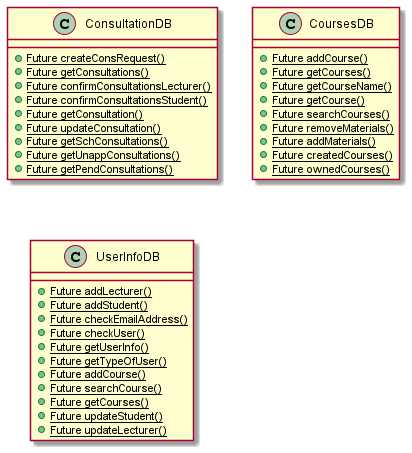
\includegraphics[scale=0.8]{dijagrami/ViewModel.PNG}
				\centering
				\caption{Dijagram razreda - dio ViewModel}
				\label{fig:ViewModel}
			\end{figure}
			
			Na slici \ref{fig:View3} su prikazani razredi koji pripadaju \textit{frontend} dijelu MVVM arhitekture. View razredi služe za prikaz podataka korisniku. Svi View razredi su implementirani kao State, što znači da se njihov prikaz osvježava sa svakom promjenom stanja razreda.
			
			Zbog lakšeg prikaza, dijagram razreda View komponente je podijeljen na tri dijela, koji su prikazani jedan ispod drugog.
			
			\eject
			\begin{figure}[h]
				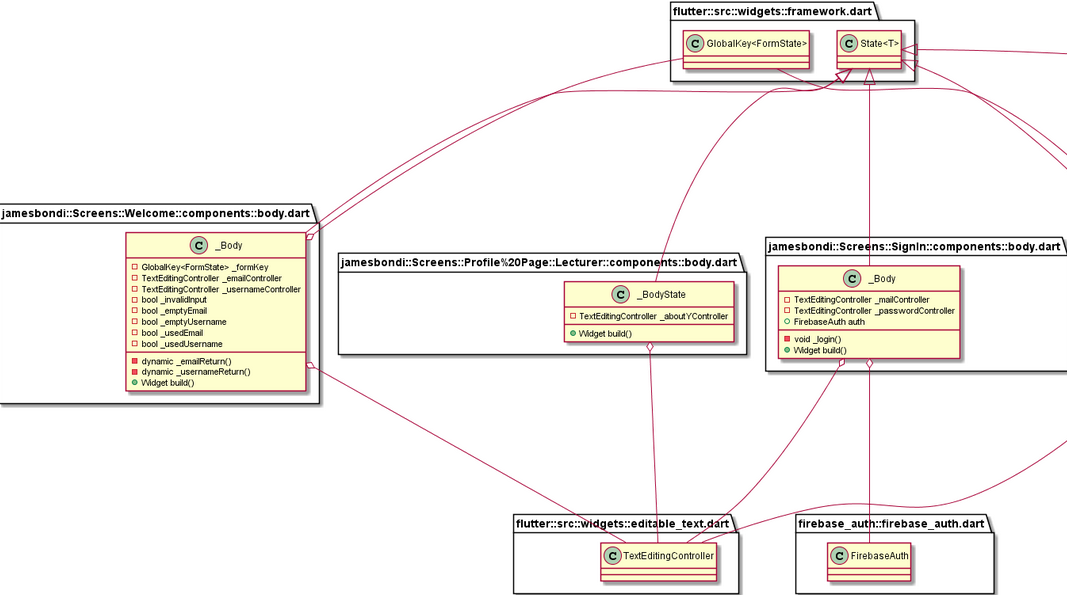
\includegraphics[scale=0.41]{dijagrami/View1.PNG}
				\centering
			\end{figure}
			
			\begin{figure}[h]
				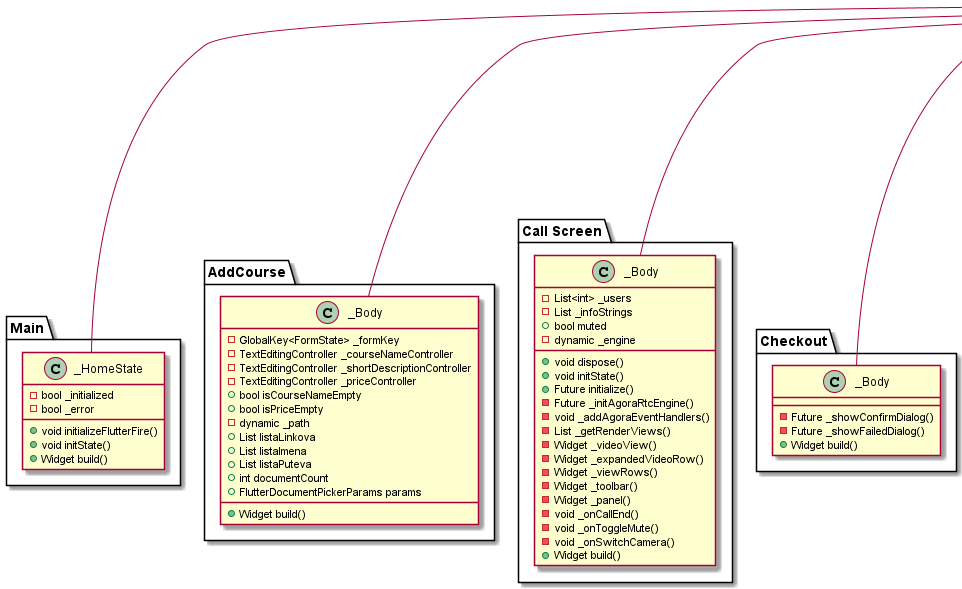
\includegraphics[scale=0.44]{dijagrami/View2.PNG}
				\centering
			\end{figure}
			
			\begin{figure}[hbt!]
				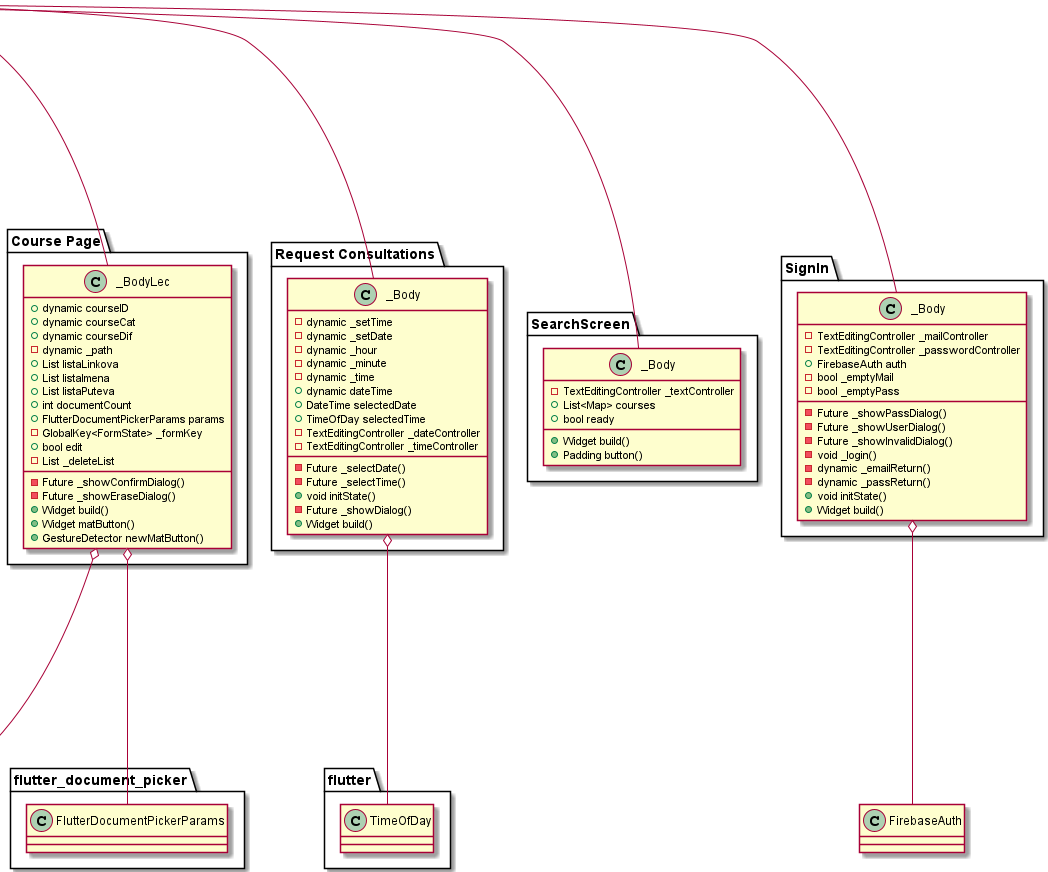
\includegraphics[scale=0.4]{dijagrami/View3.PNG}
				\centering
				\caption{Dijagram razreda - dio View}
				\label{fig:View3}
			\end{figure}
			
			\eject
			
		\section{Dijagram stanja}
			
			
			Dijagram stanja prikazuje stanja objekta te prijelaze iz jednog stanja u drugo temeljene na događajima. Na slici \ref{fig:Dijagram_stanja} prikazan je dijagram stanja za korisnika koji je registriran kao polaznik. Nakon prijave, polazniku se prikazuje početna stranica na kojoj su navedene kategorije tečajeva. Dodirom na željenu kategoriju polazniku se prikazuje izbornik u kojem odabire težinu tečaja. Aplikacija će zatim prikazati tečajeve koji zadovoljavaju zahtjeve polaznika. Pretraživanje tečajeva moguće je provesti i unosom ključnih riječi u pretraživač kojem se pristupa dodirom na "Search". Dodirom na tečaj prikazuju se njegove informacije. Ako polaznik odabere neupisani tečaj, ima opciju pregleda profila predavača i opciju upisa tečaja koji uključuje naplatu korištenjem vanjskog servisa. Odabirom već upisanog tečaja polazniku se također nudi opcija pregleda profila predavača, kao i opcija preuzimanja materijala. Dodirom na "Ask for consultations" otvara se izbornik koji omogućuje zatraživanje novog termina konzultacija.
			
			Upravljanje konzultacijama polazniku je dostupno dodirom na "Consultations". Na vrhu stranice nalazi se lista termina konzultacija dogovorenih s predavačem. Listu je moguće osvježiti dodirom na "Refresh". Videopoziv se započinje dodirom na "consultations" pokraj pripadnog dogovorenog termina. Na stranici su također prikazani termini konzultacija ponuđeni od strane predavača. Ponuđeni termin moguće je prihvatiti ili odbiti. Ako polaznik prihvati termin, on se pojavljuje u listi dogovorenih termina. U slučaju odbijanja termina, polazniku se otvara izbornik u kojem je moguće predložiti novi termin konzultacija.
			
			Dodirom na "Profile" polazniku se otvara prikaz osobnih podataka. Polaznik ima opciju izmijeniti osobne podatke dodirom na "Edit your profile", kao i opciju prikaza upisanih tečajeva dodirom na "Show owned courses". Odjava se provodi dodirom na "Sign out".
			
			\eject
			
			\begin{figure}[h]
				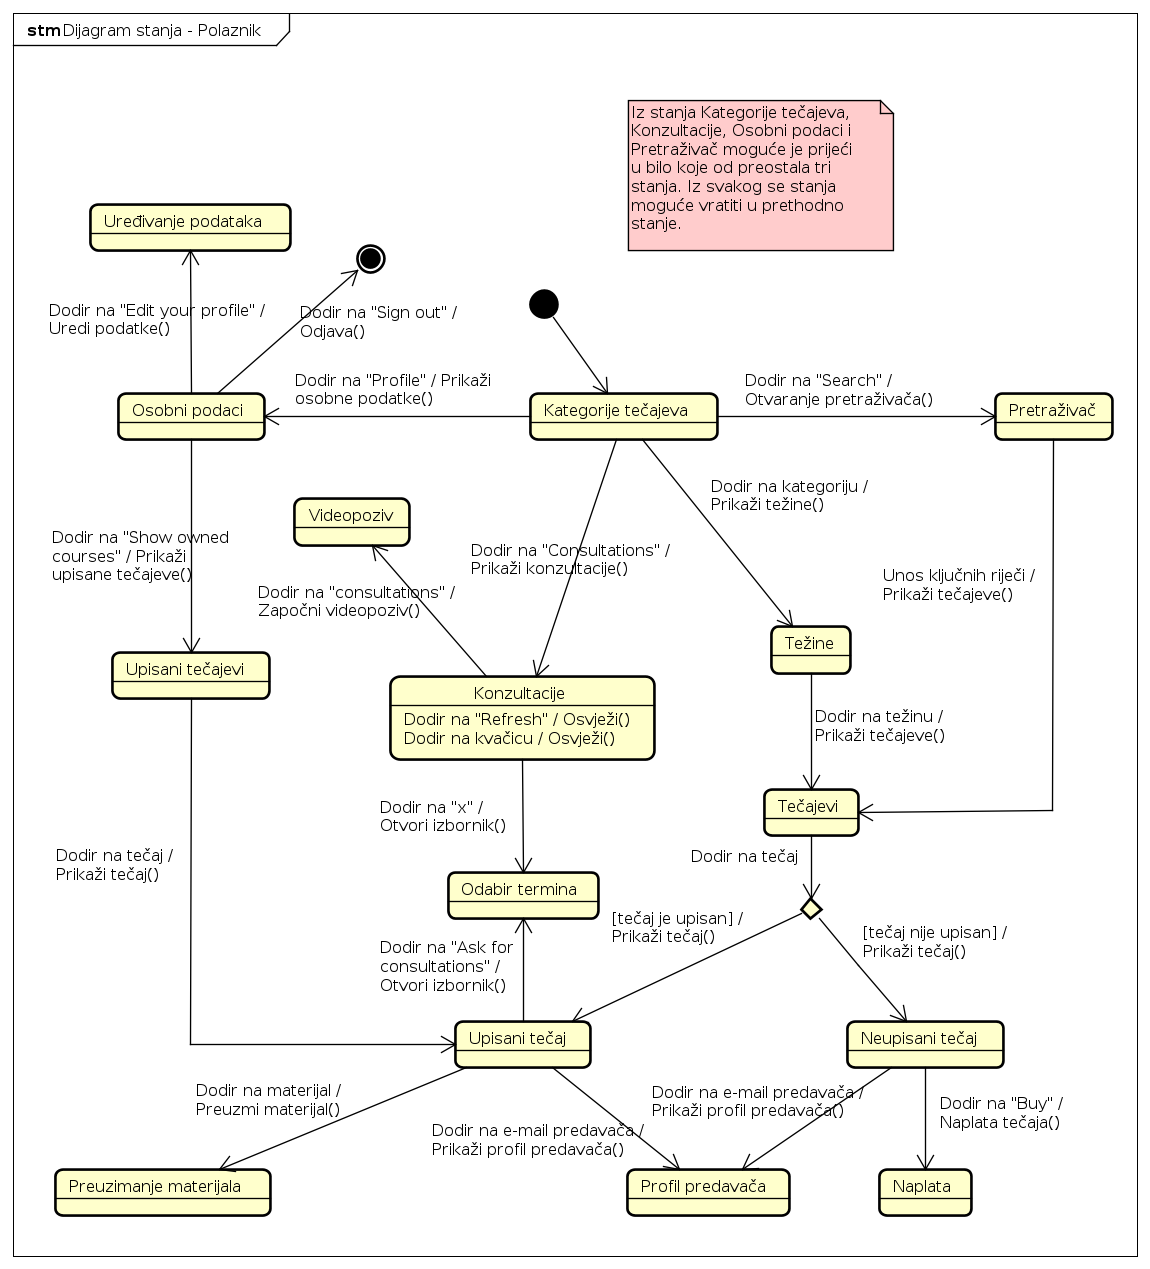
\includegraphics[scale=0.5]{dijagrami/Dijagram_stanja.PNG}
				\centering
				\caption{Dijagram stanja - Polaznik}
				\label{fig:Dijagram_stanja}
			\end{figure}
		
		
			\eject 
		
		\section{Dijagram aktivnosti}
			
			\textbf{\textit{dio 2. revizije}}\\
			
			 \textit{Potrebno je priložiti dijagram aktivnosti s pripadajućim opisom. Dijagram aktivnosti treba prikazivati značajan dio sustava.}
			
			\eject
		\section{Dijagram komponenti}
		
			Dijagram komponenti prikazuje odnos komponenti u sustavu. Na slici \ref{fig:Dijagram_komponenti} prikazana je struktura cijele aplikacije. Podaci potrebni za rad aplikacije nalaze se u NoSQL bazi podataka pohranjenoj u oblaku, kojoj se pristupa preko sučelja koje nudi Firebase. ViewModel je središnja komponenta sustava koja u sebi sadrži mapu 'components'. ViewModel koristi Flutter API, te Agora SDK za uslugu uspostavljanja videopoziva. Razredi koji služe za prikaz podataka korisniku nalaze se u mapi Screens.
			
			\begin{figure}[h]
				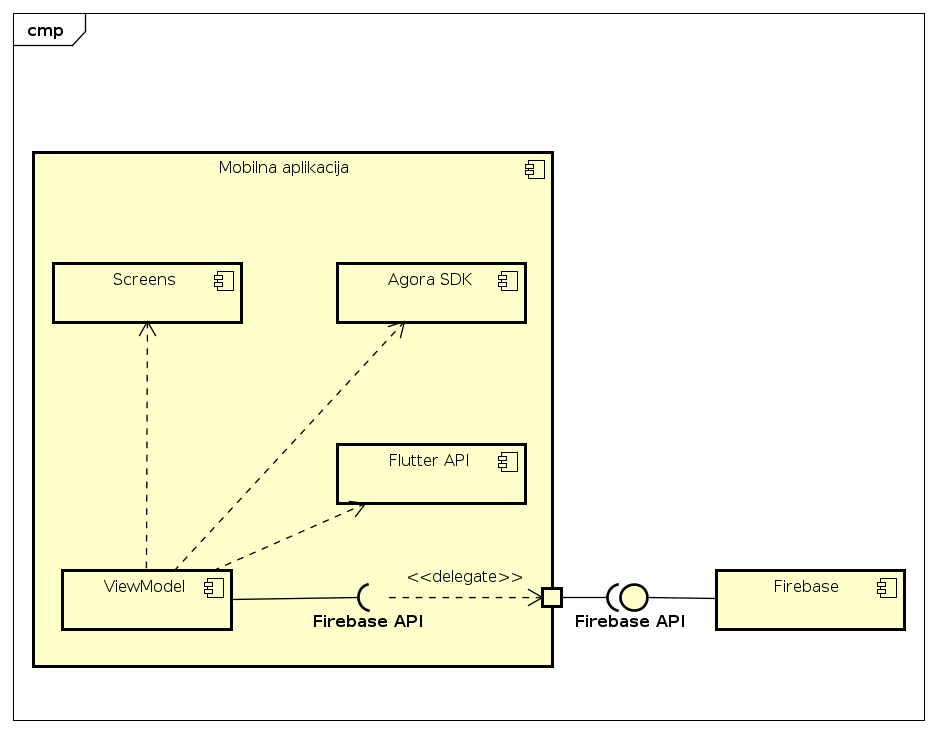
\includegraphics[scale=0.6]{dijagrami/Dijagram_komponenti.PNG}
				\centering
				\caption{Dijagram komponenti}
				\label{fig:Dijagram_komponenti}
			\end{figure}